\documentclass[11pt]{article}
\usepackage{amssymb}
\usepackage[english]{babel}
\usepackage{fullpage}
\usepackage{multirow}
\usepackage{graphicx}
\usepackage{sidecap}
\usepackage{caption}
%\usepackage{subcaption}
\usepackage{color}
\usepackage{float}
\usepackage{listings}
\usepackage[utf8]{inputenc}

\lstdefinestyle{myPython}{
	language=Python,                     % the language of the code
	basicstyle=\linespread{.9}\footnotesize,       % the size of the fonts that are used for the code
	numbers=none,                   % where to put the line-numbers
	numberstyle=\tiny\color{black},  % the style that is used for the line-numbers
	stepnumber=1,                   % the step between two line-numbers. If it's 1, each line
	% will be numbered
	numbersep=5pt,                  % how far the line-numbers are from the code
	backgroundcolor=\color{white},  % choose the background color. You must add \usepackage{color}
	showspaces=false,               % show spaces adding particular underscores
	showstringspaces=false,         % underline spaces within strings
	showtabs=false,                 % show tabs within strings adding particular underscores
	frame=single,                   % adds a frame around the code
	rulecolor=\color{black},        % if not set, the frame-color may be changed on line-breaks within not-black text (e.g. commens (green here))
	tabsize=2,                      % sets default tabsize to 2 spaces
	captionpos=b,                   % sets the caption-position to bottom
	breaklines=true,                % sets automatic line breaking
	breakatwhitespace=false,        % sets if automatic breaks should only happen at whitespace
	title=\lstname,                 % show the filename of files included with \lstinputlisting;
	% also try caption instead of title
	keywordstyle=\color{blue},      % keyword style
	commentstyle=\color{green},   % comment style
	stringstyle=\color{red},      % string literal style
	%escapeinside={\%*}{*)},         % if you want to add a comment within your code
	morekeywords={*,...}            % if you want to add more keywords to the set
	linespread=0.1 %Ecart entre les lignes <=1
}


\makeatletter

\newcommand{\rem}[1]{\fbox{\sf {#1}}}

\title{LOG8415 \\ Concepts avanc\'{e}s en infonuagique \\ TP2\\ MapReduce with Hadoop and Spark on Microsoft Azure}

\author{
	Antoine Delaite, Mohamed Amine Barrak et Philippe Troclet \\
		\\
	Travail pr\'{e}sent\'{e} \`a \\
		\\
	Foutse Khomh et S. Amirhossein Abtahizadeh \\
		\\
	D\'{e}partement G\'{e}nie Informatique et G\'{e}nie Logiciel \\
	\'{E}cole Polytechnique de Montr\'{e}al, Qu\'{e}bec, Canada
}

\date{22 mars 2017}

\begin{document}
\maketitle

\section{Introduction}

Le but de ce TP est la familiarisation de l'utilisation de la technique de MapReduce sur les Frameworks Hadoop et Spark en utilisant instance de Microsoft Azure. Tout d'abord, Hadoop doit être installé sur Ubuntu et de réaliser les configurations nécessaire afin d'exécuter les scripts de MapResuce. Par défaut, il est configuré en mode autonome "Standalone". 
\\

Plusieurs expériences doivent être effectuées en utilisant Hadoop. La première expérience consiste à exécuter WordCount sur un fichier texte dans le mode "Standalone". La deuxième expérience consiste à mesurer et comparer le temps d'exécution de WordCount sur Hadoop en mode autonome par rapport à Linux (Ubuntu). La troisième expérience consiste à analyser la performance de Hadoop et de la comparer avec celle du Framework Apache Spark MapReduce. Hadoop et Spark doivent d'abord être configurés sur une instance Azure de type D11-V2 (14G RAM, 2 cores CPU) et durant l'expérience nous analysons le temps nécessaire pour exécuter le programme de WordCount avec le fichier volumineux proposée "pg4300.txt". 
\\

Enfin, nous avons résolu un problème de Business Intelligence en utilisant une base de données volumineuse (Fichier CSV) et de répondre a une liste de question. Nous avons utilisée des programmes Python implémenté sur Spark ainsi que le principe de MapReduce et SparkSQL. Nous avons identifiée des règles pour les appliquer au données proposée afin d'identifier des anomalies dans le fichier.
%----------------------------------------------------------------------------------------
%	HADOOP VS LINUX
%----------------------------------------------------------------------------------------
\section{Hadoop}
Tout d'abord, nous avons télécharger et installer la version hadoop-2.7.3 de Hadoop. Ensuite, nous avons réaliser les configurations nécessaire afin d'utiliser hadoop.
Après l'installation, nous exécutons la commande "JPS" (Java Virtual Machine Process Status Tool) pour lister les HotSpots qui s'exécutent sur la machine virtuelle (JVM).


\begin{center}
	\begin{lstlisting}
    jps
    2176 SecondaryNameNode
    2339 ResourceManager
    2788 Jps
    2468 NodeManager
    1961 DataNode
    1802 NameNode
	\end{lstlisting}
\end{center}
Nous remarquons tout les outils nécessaires pour exécuter des programmes sur hadoop en mode distribuée sur des nœuds. Mais, suite a notre utilisation d'un seul nœud, nous avons utilise le mode standalone pour tester hadoop.
\\

$\bullet$ NameNode : c'est conu comme le maitre dans l'architechture hadoop, elle stocke dedant les metadata de HDFS. Mais le donee est stocke dans le Datanode (slave).
\\

$\bullet$ DataNode : Elle est connu comme le Slave dans l'architechture de hadoop, elle est responsable de stocker les donneees actuelle dans HDFS.
\\

Pour réaliser la première expérience, nous avons exécuter le code de WordCount, qui permet de retourner l'occurrence de chaque mot dans un fichier.
Nous avons utiliser le fichier pg4300 (livre de James Joyce) \cite{wwwguten70} comme données d'entrée pour le script Wordcount. Le principe WordCount est base sur le mécanisme de MapReduce dans lequel ont cherche les données sous forme de $<$ key, valeur$ >$, le "key" c'est l'objet qu'on va chercher et "valeur" sa valeur trouvée. Dans un premier temps, il réalise le Mapping c'est a dire de chercher les mots rencontre dans chaque ligne et de mettre son occurrence. Ensuite, il réalise la phase de Reduce qui collecte les mots trouvées pour chaque ligne et additionne les occurrence. Enfin, il t'affiche le résultat d'occurrence de chaque mot dans le fichier donnée en entrée.
\\
Nous avons utiliser la commande suivante pour executer l'exemple java de WordCount:
\\

\begin{scriptsize} 
hadoop jar share/hadoop/mapreduce/hadoop-mapreduce-examples-2.7.3.jar wordcount /usr/pg4300.txt /output/mr
\end{scriptsize}
\\

Ceci est une capture du résultat de l'exécution de WordCount sur Hadoop:
\\
\begin{scriptsize}
  \begin{lstlisting}
        youngster	2
        youngsters,1
        youngun.	1
        your	451
        your.	1
        your?	4
        youre	8
        yourn	1
        yours	8
        yours,	4
        yours.	2
        yours?	2
        yourself	14
        yourself!	1
        yourself,	3
        yourself.	12
        yourself?	8
        yourselves 1
        yourselves. 1

  \end{lstlisting}
\end{scriptsize}
%----------------------------------------------------------------------------------------
%	Comparaison hadoop et linux
%----------------------------------------------------------------------------------------
\section{Comparaison du temps d'exécution entre Hadoop ,Linux et Spark}
Comme mentionné dans la partie précédente, hadoop a été installé sur une
instance D11-V2 d'Azure. Nous avons installée aussi spark. Nous allons tester
la duree de temps parcourue par les deux Framework ainsi que Linux. Nous avons
utilise le programme "wordcount" base sur MapReduce et de l'exécuter sur le
fichier a été exécuté sur le seul fichier pg4300 \cite{wwwguten70}. Nous
avons mi le fichier dans la HDFS, ensuite, a l'aide d'un \textbf{Script}, nous
avons réaliser une exécution 10 fois pour chaque des plate forme et stocker le
temps écoulée dans des fichiers. 

Comme il est connu, les systèmes distribuée son plus rapide que le système d'exploitation seul (Ubuntu). 


\subsection{Résultats}

% Présentation des graphiques / tableaux
Les résultats n'ont pas progressé comme prévu. Étonnamment, linux a effectué les tâches entre 5 fois plus vite que hadoop. Nous avons enregistre que Linux prend en moyenne 0.832 secondes ainsi que Hadoop avec 4.173 secondes et enfin Spark avec 6.456 secondes. La figure \ref{fig:CF1} montre nos expériences avec 10 itération pour toute plateforme (Ubuntu, Spark et Hadoop) et le temps écoulée pour chacune pour terminer la tache.

\begin{figure}
    \centering
    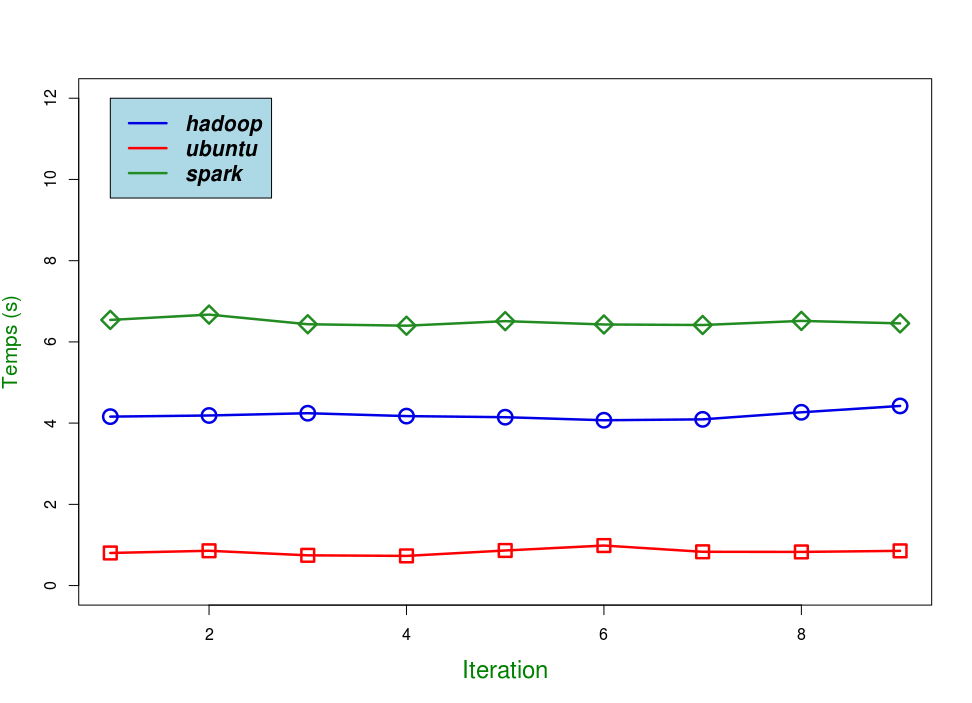
\includegraphics[width=1\textwidth]{images/ada.png}
    \captionof{figure}{Comparaison de performance hadoop, spark et ubuntu}
    \label{fig:CF1}
\end{figure}
\subsection{Analyse}

% Analyse des résultats, ce qui est surprenant
Les résultats inattendus nous ont fait curieux de chercher des raisons. En fait, comme nous le savons, Hadoop et Spark ont été développé pour être exécuter sous une architecture distribuée de nœud ainsi avec une grande quantité de données (Big Data). Or ce n'est pas le cas avec notre exemple. Comme le montre la recherche, Hadoop et Spark ne sont pas vraiment adapté à une petite quantité de données. Il existe plusieurs solutions qui exécutent des tâches plus rapidement que Hadoop et Spark sur des gigaoctets de données. En fait, Hadoop et Spark devraient effectuer certaines tâches derrière la scène pour commencer. Comme le montrent nos résultats d'expériences que Ubuntu est plus rapide que Spark et Hadoop.

\pagebreak
%----------------------------------------------------------------------------------------
%	Analyse de donneee
%----------------------------------------------------------------------------------------
\section{Questions}
Pour répondre aux différentes questions nous avons utlisé le langage python et
spark-submit. Nos scripts se trouvent dans le répertoire TP2/Scripts du dépôt
GIT. Nous sommes principalement référé à \cite{SparkDoc} pour avoir des
exemples d'utilisation. Nous avons utilisé les mapReduce classique, des map
avec la variante reduceByKey pour regrouper les lignes selon une clef. 
Les scripts se décomposent en général comme suit: \\
On charge le contexte de Spark et le contexte SQL:
\begin{verbatim}
spark = SparkContext.getOrCreate()
sqlContext = SQLContext(spark)
\end{verbatim}
Puis on transforme le fichier d'entrée en base de données SQL, ce qui
convertit aussi les type en type du langage, par exemple en Datetime
ou en boolean pour les champs date et vip.:
\begin{verbatim}
	df = sqlContext.read.load(input_path,
		format='com.databricks.spark.csv',
		header='true', inferSchema='true')
\end{verbatim}

Les opérations sur la base de données sont très pratiques car on peut
manipuler les champs aisément, ceux-ci étant précisé dans le header du 
ficheir, et que les types ont été convertis.
Cependant on ne peut pas effectuer directement d'opération MapReduce sur
un objet de type base de données (dataframe), mais celui ci a un champ
rdd qui permet de combiner les opérations MapReduce facilement tout en 
ayant accès aux champs. Un exemple parlant permettant de créer très
facilement un tuple clef-valeur:
\begin{verbatim}
df.rdd.map(lambda purchase: (purchase.member_id, purchase.date))
\end{verbatim}

Pour lancer une opération il faut lancer la commande suivante, pour la
question 6 par exemple:
\begin{center}
\begin{verbatim}
	spark-submit Q6_max_price.py ../Data/data_dump.csv 2> err.txt
\end{verbatim}
\end{center}

\subsection*{Q1: How many distinct members are included in the data set?}
	Pour cette question nous avons utlisé la requête SQL groupBy selon
	le champ member\_id puis nous comptons les lignes obtenues.\\
	\textbf{Réponse:\\}
	Nous trouvons qu'il y a 2500 membres distincts.
\subsection*{Q2: When did the first purchase happen?}
	Pour cette question nous avons aussi utilisé une requête SQL, en
	ordonnant par rapport au champ data avec orderBy.\\
	\textbf{Réponse:\\}
	Le premier achat retrouvé dans les logs a eu lieu le 2007-12-02.

\subsection*{Q3: What are the different card types used in purchasing?}
	Pour cette question nous avons effectué un distinct sur la base
	de données selon le champ card\_type.\\
	\textbf{Réponse:\\}
	Nous trouvons 16 types de carte différentes:
	\begin{center}
	\begin{tabular}{|c|c|c|c|}
		\hline
		jcb & visa-electron & maestro & diners-club-international \\
		\hline
		solo & americanexpress & diners-club-enroute & china-unionpay \\
		\hline
		bankcard & switch & mastercard & instapayment \\
		\hline
		visa & diners-club-carte-blanche & diners-club-us-ca & laser \\
		\hline
	\end{tabular}
	\end{center}
\subsection*{Q4: How many VIP members do we have in our data set?}
	Pour cette question nous avons fait deux MapReduce en série, le
	premier crée un tuple clef-valeur $(customer\_id, (data, vip)$ afin
	de pouvoir faire un reduceByKey qui nous donne la ligne d'achat 
	la plus récente associé à cette id. Enfin nous remappons afin de
	n'obtenir que champ vip de la valeur et nous réduisons en sommant
	pour chaque vip=True.\\
	\textbf{Réponse:\\}
	En date nous avons 1245 membres VIP.\\
\subsection*{Q5: How many Canadian female members purchased an item from Zone7?}
	Pour cette question une série de filter sur la base SQL nous donne
	le résultat.\\
	\textbf{Réponse:\\}
	Nous avons trouvé 16 femmes canadiennes ayant effectué un achat dans la
	zone 7.
\subsection*{Q6: Which item has the maximum amount of price?}
	Pour cette question nous trions en ordre décroissant la base données
	selon le champ amount et récupérons la première entrée.\\
	\textbf{Réponse:\\}
	Le produit le plus cher en vente à le numéro de série 330092, et à pour
	valeur 9999.87\$.
\subsection*{Q7: What are the top 3 countries from which people made purchases?}
	Pour cette question nous avons fait un groupBy par indicatif de pays
	et sommé le nombre d'entrée et ensuite nous avons trié et affiché
	les 3 premières entrées.\\
	\textbf{Réponse:\\}
	Les 3 pays dans lesquels il y a eu le plus de ventes sont:
	\begin{center}
	\begin{tabular}{|c|c|}
		\hline
		Indicatif du pays & nombre de ventes \\
		\hline
		CN & 4623 \\
		\hline
		ID & 2695 \\
		\hline
		RU & 1415 \\
		\hline
	\end{tabular}
	\end{center}
\subsection*{Q8: What are the relevant patterns for each column of the dataset?}
	La première colonne est la colonne member\_id, nous avons remarqué qu'un
	id est composé de 6 chiffres commençant par 10. Nous utilisons la 
	fonction suivante basée sur une regexp:
	\begin{lstlisting}[style=myPython]
	def check_member(member):
		reg = "\A10\d{4}\Z"
		if not(re.match(reg, str(member))):
			return False
		return True
	\end{lstlisting} 
	La deuxième colonne correspond à la date, on s'assure que la date est
	postérieure aux années 2000 et au plus tard 2017. Il faut aussi
	vérifier que les jours et les mois sont corrects par exemple,
	notamment les années bisextiles.
	\begin{lstlisting}[style=myPython]
	def check_date(date):
		reg="(200[0-9]|201[0-7])-(0\d|1[0-2])-(0\d|[12]\d|3[0-1])"
		if not(re.match(reg, date)):
			return False
		# Feb and bisextile years
		res = re.match("(....)-02-(..)", date)
		if (res):
			year = int(res.group(1))
			day = int(res.group(2))
			if (day > 29 or (day==29 and year%4!=0)):
				return False
		return True
	\end{lstlisting}
	La troisième colonne correspond à l'indicatif du pays, nous avons 
	récupéré en ligne une liste \cite{indicPays} afin de vérifier que
	les indicatifs sont corrects:
	\begin{lstlisting}[style=myPython]
	def check_country(country):
	all_country_code = [ ... ]
		if country in all_country_code:
			return True
		else:
			return False
	\end{lstlisting}
	La quatrième colonne correspond au genre de l'acheteur, soit homme
	ou femme. Une regexp simple permet de vérifier ce champ:
	\begin{lstlisting}[style=myPython]
	def check_gender(gender):
		reg = "\A(Male|Female)\Z"
		if not(re.match(reg, gender)):
			return False
		return True
	\end{lstlisting}
	La cinquième colonne correspond à l'adresse IP, nous vérifions
	qu'il y a bien quatre fois 1 à 3 chiffres séparés par des points.
	Chacune des valeurs devant être entre 0 et 255. 
	\begin{lstlisting}[style=myPython]
	def check_ip_adr(adr):
		reg = "\A(\d{1,3})\.(\d{1,3})\.(\d{1,3})\.(\d{1,3})\Z"
		bytes = re.match(reg, adr)
		isValid = True
		for i in range(1,5):
			tmpbyte = bytes.group(i)
			#many values use 255 and 0 so they must be legit
			isValid = isValid and (int(tmpbyte) <= 255) and (int(tmpbyte) >= 0)
		return isValid
	\end{lstlisting}
	La sixième colonne correspond à la valeur de l'achat, nous vérifions
	à l'aide de la regexp qu'il est positif et que le montant est à
	3 ou 4 chiffres avec 2 chiffres après la virgule:
	\begin{lstlisting}[style=myPython]
	def check_amount(amount):
		reg = "\A$\d+\.\d{1,2}\Z"
		if re.match(reg, amount):
			return True
		else:
			return False
	\end{lstlisting}
	La septième colonne consiste à vérifier que le booléen vip est soit
	vrai ou faux, c'est très semblable à Male|Female. \\
	La huitième colonne contient les product\_id, il faut vérifier qu'il
	commence par 330 et contient bien 6 chiffres:
	\begin{lstlisting}[style=myPython]
	def check_product_id(product_id):
		#peut on faire mieux? FIXME
		#is it usefull to perform check if it is already an int?
		reg = "\A330\d{3}\Z"
		if re.match(reg, str(product_id)):
			return True
		else:
			return False
	\end{lstlisting}
	Pour la neuvième colonne, le type de carte, il n'y a pas de pattern
	prédéfini, nous avons vérifié que les types de carte de la question
	3 semblaient correct et nous les avons utilisé pour filtrer
	cette colonne.
	La dixième colonne correspond à un numéro sérial, décomposé en 3,
	on vérifie qu'il y a 3chiffres-2chiffres-4chiffres.
	\begin{lstlisting}[style=myPython]
	def check_serial(serial):
		reg = "\d{3}-\d{2}-\d{4}$"
		if re.match(reg, serial):
			return True
		else:
			return False
	\end{lstlisting}
	Enfin la dernière colonne la dixième, correspond à la zone et il faut
	simplement vérifier que le pattern est bon:
	\begin{lstlisting}[style=myPython]
	def check_zone(zone):
		reg = "zone[1-7]$"
		if re.match(reg, zone):
			return True
		else:
			return False
	\end{lstlisting}

\subsection*{Q9: There are three rows in the dataset that can be identified as anomaly}
	Il y a trois anomalies dans les données et nous avons trouvé les trois
	\begin{itemize}
		\item La première anomalie est dûe à l'adresse ip et la valeur 777 qui n'est
	pas valide.\\
	\begin{lstlisting}[style=myPython]
	Row(member_id=102169, date=datetime.datetime(2016, 5, 10, 0, 0), country=u'CA', gender=u'Female', ip_address=u'164.176.777.46', amount=u'$7338.41', vip=True, product_id=330082, card_type=u'jcb', serial=u'417-94-9025', zone=u'zone6')
	\end{lstlisting}
		\item La deuxième est liée au serial, le dernier nombre 99000 a un chiffre en
	trop.\\
	\begin{lstlisting}[style=myPython]
	Row(member_id=100216, date=datetime.datetime(2015, 2, 1, 0, 0), country=u'CN', gender=u'Male', ip_address=u'151.210.200.198', amount=u'$6835.26', vip=False, product_id=330090, card_type=u'jcb', serial=u'425-18-99000', zone=u'zone7')
	\end{lstlisting}
		\item La troisième anomalie a été plus dure à trouver car elle était masquée
	par la conversion automatique de la date en type python datetime lors du
	sqlContext.read.load(...). Pour pouvoir travailler sur les string brute
	il faut mette l'option inferSchema à False. L'anomalie correspondait
	donc à la date dont le jour écrit avec un seul chiffre: 1 au lieu de 01.
	\begin{lstlisting}[style=myPython]
	Row(member_id=u'100379', date=u'2011-06-1', country=u'MN', gender=u'Female', ip_address=u'5.142.225.113', amount=u'$1053.09', vip=u'false', product_id=u'330113', card_type=u'laser', serial=u'177-29-7433', zone=u'zone2')
	\end{lstlisting}
	\end{itemize}
\section{Conclusion}
	Grâce à ce TP nous avons pu apprendre à mettre en place des outils
	très utilisés dans les cluster des cloud provider où même des cloud
	privés. Ces outils correspondent à hadoop et spark fonctionnant
	au dessus d'hadoop et permettant des optimisations. \\
	Nous avons comparé les performances et vu qu'en local il n'y avait
	évidemment pas de réel gain à utiliser hadoop ou spark. \\
	Cependant lors de la deuxième partie du TP nous avons 
	manipulé les MapReduce et avons noté que l'implémentation est
	condensé, plutôt facile et efficace. \\
	Nous avons pu effectuer diverses opérations classique qui dans un
	cas d'utilisation réel aurait été effectué sur un grand nombre de noeud
	sur des ensembles de fichiers beaucoup plus gros.

%\section{Références:}
% https://doc.ubuntu-fr.org/dd
% https://romanrm.net/dd-benchmark
%\subsection{Spark}
%\begin{itemize}
%	\item http://spark.apache.org/examples.html
%\end{itemize}

\bibliographystyle{IEEEtran}
\bibliography{rapport}

\end{document}
